\subsection{UC3 - Manipolazione del dataset}
\label{uc3}

    \begin{figure}[htbp]
        \centering
        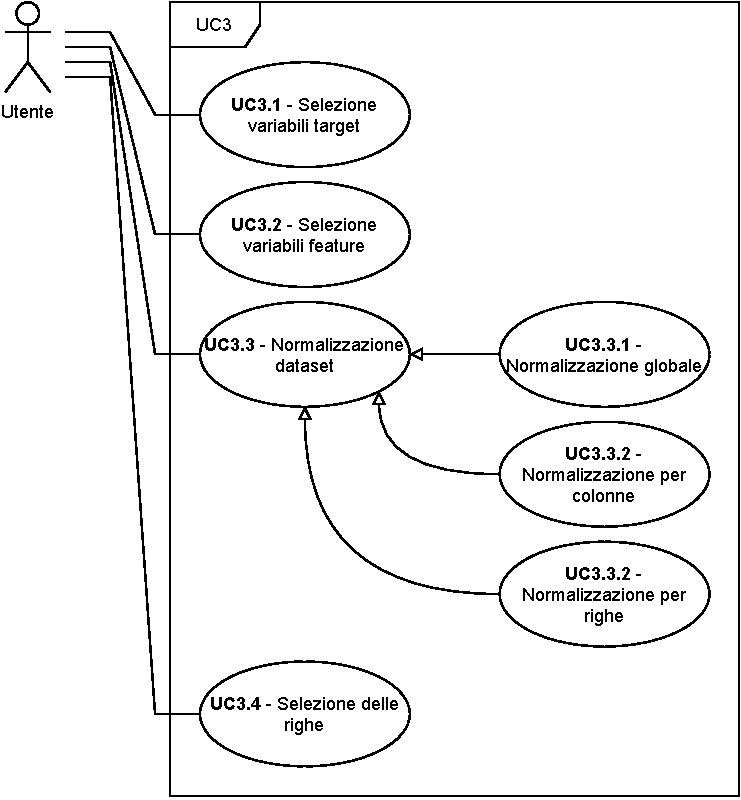
\includegraphics[width=0.7\textwidth]{source/sections/casi-uso/diagrams/uc3.pdf}
        \caption{UC3 - Manipolazione del dataset}
        \label{fig:uc3}
    \end{figure}
    
    \begin{itemize}
    \item \textbf{Attore}: utente;
    \item \textbf{Descrizione}: L'utente può modificare il dataset che ha caricato, modificandone i valori 
    \item \textbf{Precondizione}:
    \begin{itemize}
        \item eseguito l'upload del dataset come matrice $N\times M$ (\hyperref[uc2]{UC2});
    \end{itemize}
    \item \textbf{Postcondizione}: dataset modificato secondo le intenzioni dell'utente
    \item \textbf{Scenario Principale}: 
    \begin{enumerate}
        \item l'utente modifica il dataset a seconda delle funzionalità disponibili
    \end{enumerate}  
    \end{itemize}


    \subsubsection{UC3.1 - Selezione delle variabili target}
    \label{uc3.1}
    \begin{itemize}
    \item \textbf{Attore}: utente;
    \item \textbf{Descrizione}: L'utente sceglie quali, tra le variabili del dataset, considerare come variabili target;
    \item \textbf{Precondizione}:
    \begin{itemize}
        \item eseguito l'upload del dataset come matrice $N\times M$ (\hyperref[uc2]{UC2});
    \end{itemize}
    \item \textbf{Postcondizione}: le features selezionate verranno considerate dal sistema come variabili target;
    \item \textbf{Scenario Principale}: 
    \begin{enumerate}
        \item l'utente visualizza le features del dataset;
        \item seleziona le features del dato che vuole considerare come variabili target;
    \end{enumerate}  
    \end{itemize}
    
    \subsubsection{UC3.2 - Selezione delle features}
    \label{uc3.2}

    \begin{itemize}
    \item \textbf{Attore}: utente;
    \item \textbf{Descrizione}: l'utente seleziona le features del dataset è interessato a visualizzare;
    \item \textbf{Precondizione}: 
     \begin{itemize}
        \item eseguito l'upload del dataset come matrice $N\times M$ (\hyperref[uc1]{UC1});
    \end{itemize}
    \item \textbf{Postcondizione}: la matrice contiene $M-i$ colonne, dove $i$ è il numero di features che l'utente ha scartato;
    \item \textbf{Scenario Principale}: 
    \begin{enumerate}
        \item l'utente visualizza le features del dataset, che corrispondono alle colonne della matrice;
        \item l'utente seleziona le feature a cui è interessato;
    \end{enumerate}
    \end{itemize}
    
    \subsubsection{UC3.3 - Normalizzazione del dataset}
    \label{uc3.3}
    
    \begin{itemize}
    \item \textbf{Attore}: utente;
    \item \textbf{Descrizione}: un dataset può contenere dati non normalizzati, normalizzare il dataset può risultare utile per una migliore visualizzazione dei dati;
    \item \textbf{Precondizione}: 
    \begin{itemize}
        \item eseguito l'upload del dataset come matrice $N\times M$ (\hyperref[uc1]{UC1});
    \end{itemize}  
    \item \textbf{Postcondizione}: il dataset contenente dati non normalizzati viene normalizzato a seconda del tipo di normalizzazione scelto;
    \item \textbf{Scenario Principale}:
    \begin{enumerate}
        \item l'utente seleziona l'opzione di normalizzazione e specifica quale desidera effettuare;
    \end{enumerate}  
    \item \textbf{Generalizzazioni}: 
     \begin{enumerate}
            \item l'utente sceglie su quale subset di dati effettuare la normalizzazione:
                \begin{enumerate}
                    \item normalizzazione Globale (\hyperref[uc3.3.1]{UC3.3.1});
                    \item normalizzazione per Colonna (\hyperref[uc3.3.2]{UC3.3.2});
                    \item normalizzazione per Riga (\hyperref[uc3.3.3]{UC3.3.3}).
                \end{enumerate}
        \end{enumerate}  
    \end{itemize}
    
    \paragraph{UC3.3.1 - Normalizzazione globale del dataset}
    \label{uc3.3.1}
    \begin{itemize}
    \item \textbf{Attore}: utente;
    \item \textbf{Descrizione}: un dataset può contenere dati non normalizzati; normalizzare il dataset può risultare utile per una migliore visualizzazione dei dati, in questo caso la normalizzazione viene fatta su tutto il dataset;
    \item \textbf{Precondizione}: 
    \begin{itemize}
        \item eseguito l'upload del dataset come matrice $N\times M$ (\hyperref[uc1]{UC1});
    \end{itemize}  
    \item \textbf{Postcondizione}:  ogni valore ${x_i}_j$ del dataset viene sostituito da $ {y_i}_j = \frac{{x_i}_j - \mu}{\sigma}$ dove $\mu$ è la media dei valori presenti nel data set e $\sigma$ la loro varianza;
    \item \textbf{Scenario Principale}: 
    \begin{enumerate}
        \item l'utente seleziona l'opzione di normalizzazione e specifica che desidera una Normalizzazione Globale.
    \end{enumerate}  
    \end{itemize}
    
    \paragraph{UC3.3.2 - Normalizzazione per colonna del dataset}
    \label{uc3.3.2}
    \begin{itemize}
    \item \textbf{Attore}: utente;
    \item \textbf{Descrizione}: un dataset può contenere dati non normalizzati; normalizzare il dataset può risultare utile per una migliore visualizzazione dei dati, in questo caso la normalizzazione viene fatta colonna per colonna;
    \item \textbf{Precondizione}: 
    \begin{itemize}
        \item Eseguito l'upload del dataset come matrice $N\times M$ (\hyperref[uc1]{UC1}).
    \end{itemize}  
    \item \textbf{Postcondizione}: Ogni valore ${x_i}_j$ del dataset viene sostituito da $ {y_i}_j = \frac{{x_i}_j - \mu}{\sigma}$ dove $\mu$ è la media dei valori presenti nella colonna $j$ e $\sigma$ la loro varianza sotto radice.
    \item \textbf{Scenario Principale}: 
    \begin{enumerate}
        \item l'utente seleziona l'opzione di normalizzazione e specifica che desidera una Normalizzazione per Colonna. 
    \end{enumerate}  
    \end{itemize}
    
    \paragraph{UC3.3.3 - Normalizzazione per riga del dataset}
    \label{uc3.3.3}
    \begin{itemize}
    \item \textbf{Attore}: utente;
    \item \textbf{Descrizione}: un dataset può contenere dati non normalizzati; normalizzare il dataset può risultare utile per una migliore visualizzazione dei dati, in questo caso la normalizzazione viene fatta riga per riga;
    \item \textbf{Precondizione}: 
    \begin{itemize}
        \item eseguito l'upload del dataset come matrice $N\times M$ (\hyperref[uc1]{UC1});
    \end{itemize}  
    \item \textbf{Postcondizione}: ogni valore ${x_i}_j$ del dataset viene sostituito da $ {y_i}_j = \frac{{x_i}_j - \mu}{\sigma}$ dove $\mu$ è la media dei valori presenti nella riga i e $\sigma$ la loro varianza sotto radice;
    \item \textbf{Scenario Principale}: 
    \begin{enumerate}
        \item l'utente seleziona l'opzione di normalizzazione e specifica che desidera una Normalizzazione per riga.
    \end{enumerate}  
    \end{itemize}
    
    \subsubsection{UC3.4 - Selezione delle righe}
    \label{uc3.4}
    \begin{itemize}
    \item \textbf{Attore}: utente;
    \item \textbf{Descrizione}: L'utente sceglie le righe del dataset da considerare per la visualizzazione.
    \item \textbf{Precondizione}:
    \begin{itemize}
        \item eseguito l'upload del dataset come matrice $N\times M$ (\hyperref[uc2]{UC2});
    \end{itemize}
    \item \textbf{Postcondizione}: il dataset conterrà solo le righe specificate dall'utente
    \item \textbf{Scenario Principale}: 
    \begin{enumerate}
        \item l'utente visualizza le righe del dataset;
        \item seleziona le righe del dataset che è interessato a visualizzare;
    \end{enumerate}  
    \end{itemize}
    